\documentclass[12pt]{article}

\usepackage[utf8]{inputenc}
\usepackage[colorlinks=true, linkcolor=blue, urlcolor=blue, citecolor=blue]{hyperref}
\usepackage{amssymb}
\usepackage{amsmath}
\usepackage{graphicx}
\usepackage{titlesec}
\usepackage{tcolorbox}
\usepackage{caption}
\usepackage{titling}
\usepackage{circuitikz}
\usepackage{enumitem}
\usepackage{wrapfig}
\usepackage{float}
\usepackage{pgfplots}
%\usepackage{hyperref}
\usepackage{listings}
\usepackage{xcolor}


\definecolor{bg}{rgb}{0.1,0.1,0.1}
\definecolor{codegreen}{rgb}{0,0.8,0.2}
\definecolor{codepurple}{rgb}{0.7,0.2,0.8}
\definecolor{codeblue}{rgb}{0.2,0.6,1.0}
\definecolor{codeorange}{rgb}{0.86274509803921568627450980392157,0.86274509803921568627450980392157,0.66666666666666666666666666666667}
\definecolor{bracketcolor}{rgb}{0.2,0.73,0.69019607843137254901960784313725}

\lstdefinelanguage{PythonCustom}{
    language=Python,
    morekeywords={for,while,if,else,elif,import,from,as,def,class,return},
    morekeywords=[2]{np, arange, mean, zeros, ones, linspace}, % np functions highlighted differently
    sensitive=true,
    morecomment=[l]{\#},
    morestring=[b]',
    morestring=[b]"
}

\lstset{
    backgroundcolor=\color{bg},
    basicstyle=\ttfamily\color{white},
    keywordstyle=\color{codeblue}\bfseries,
    keywordstyle=[2]\color{codeorange}\bfseries, % second keyword set color (np functions)
    commentstyle=\color{codegreen}\itshape,
    stringstyle=\color{codepurple},
    numbers=left,
    numberstyle=\tiny\color{gray},
    breaklines=true,
    frame=single,
    language=PythonCustom,
    showstringspaces=false,
    % Coloring brackets manually
    literate=
    *{[}{{\color{bracketcolor}[}}1
     {]}{{\color{bracketcolor}]}}1
     {(}{{\color{bracketcolor}(}}1
     {)}{{\color{bracketcolor})}}1
     {=}{{\color{codeorange}=}}1
     {+}{{\color{codeorange}+}}1
     {-}{{\color{codeorange}-}}1
     {*}{{\color{codeorange}*}}1
}

\newcommand{\LaTeXs}{\LaTeX{\/} }
\newcommand{\matlabs}{{\sc Matlab{\/} }}
\newcommand{\matlab}{{\sc Matlab}}
\begin{document}

\title{Aproximarea unei melodii folosind mai multe metode de calcul numeric}

\author{
  Popa Mircea Alexandru \\
  Sîrghe Matei Ștefan \\ 
  Ungureanu Robert Afton
}

\maketitle

\section{Modelul matematic}\label{Modelul}
\begin{itemize}
\item Modelul ales de noi începe de la orice fișier audio de tip .wav, 16 bitrate, mono.\\
\item Fișierul audio poate să fie interpretat ca o amplitudine în funcție de timp. Astfel, putem să ne imaginăm că avem o funcție de tipul $f(t)$, unde $t$ este timpul și $f(t)$ este amplitudinea sunetului la acel moment.\\
\item Ca să interpretăm funcția cu acuratețe mai mare, vom aplica Short-Time Fourier Transform, care ne va permite să vedem frecvențele care compun sunetul.\\
\item Astfel o sa ajungem cu o functie $F(\tau,\omega)$ pe care o împărțim în matricea $A$ care conține modulul părții reale și matricea $\varphi$ care conține coeficientul de unghi. \\
\item Vom aplica SVD (Singular Value Decomposition) pe matricea $F(\tau,\omega)$. Factorizarea QR va fi folosită  ca să descompună $A$ în valori proprii.\\
\item Am aplicat SVD, vom obține matricea $A \approx U \Sigma V^T$, unde $U$ și $V$ sunt matricile ortogonale și $\Sigma$ este o matrice diagonală cu valorile pozitive.\\
\item Inmulțim cele 3 matrici, obținem o aproximare la matricea originală $B$ care este interpretată ca funcția $G(\tau,\omega)$. \\ 
\item Cu funcția $G(\tau,\omega)$ vom calcula Short-Time Fourier Transform inversă, care ne va permite să obținem o nouă funcție $g(t)$, aproximarea funcției originale $f(t)$.\\
\item Cu aproximarea $g(t)$ vom putea să obținem un nou fișier audio .wav, care este o aproximare a fișierului original.\\
\end{itemize}

\begin{equation}
\begin{cases}
F(\tau,\omega) = \Sigma_{t=0}^{N-1} f(t) w(t-\tau) e^{-i\omega t} \\[6pt]
Z_{i,j} = F(i,j) , Z \in \mathbb{M}_{N,M} (\mathbb{C}) \\[6pt]
A = \left| Z \right|, A \in \mathbb{M}_{N,M} (\mathbb{R}) \\[6pt]
\forall z_{n,m}=a_{n,m}+ib_{n,m} \in Z,  n \in [0,N] m \in [0,M], \exists \theta_{n,m}=\tan^{-1}(\dfrac{b_{n,m}}{a_{n,m}})\\[6pt]
\varphi = \begin{bmatrix}
\theta_{1,1} & \theta_{1,2} & ... & \theta_{1,N} \\
\theta_{2,1} & \theta_{2,2} & ... & \theta_{2,N} \\
... & ... & ... & ... \\
\theta_{M,1} & \theta_{M,2} & ... & \theta_{M,N}\\
\end{bmatrix}\\[6pt]
A \approx U\Sigma V^{*} = \Sigma_{i=1}^{k}\sigma_{i}u_{i}v_{i}^{*} = B \\[6pt] 
G(i,j) = B_{i,j} + \varphi_{i,j} , B \in \mathbb{M}_{N,M} (\mathbb{C}) \\[6pt]
g(t) = \frac{1}{w(t-\tau)} \frac{1}{2\pi} \Sigma_{\omega=0}^{N-1} G(\tau,\omega) e^{+i\omega t} \\[6pt]
%w(n)=\frac{1}{2}[1+cos(\frac{2\pi n}{L})] , w:\mathbb{R} \rightarrow \mathbb{R} \\[6pt]
\end{cases}
\end{equation}

\subsection{Discretizarea domeniului}\label{methods}

Domeniul este reprezentat de catre durata melodiei care este înmultită cu sampling rate-ul de 44100 Hz.

\begin{equation}
N = \text{l} \times h
\end{equation}

\begin{itemize}
	\item $l$ este durata melodiei în secunde.
    \item $h$ este sampling rate-ul default de 44100 Hz.
    \item $M$ este numărul de frecvențe pe care îl conține o melodie.
\end{itemize}

\subsection{Transformata Fourier}\label{Modelul}

Teoretic vorbind, Short-Time Fourier Transform este:
\begin{equation}
    F(\tau,\omega)=\int_{-\inf}^{+\inf}f(t)w(t-\tau)e^{-i\omega t}dt
\end{equation}
 dar funcția $f(t)$ este discretizată, deci vom folosi transformarea discretă ca să calculăm $F(\tau,\omega)$.

\begin{equation}
    F(\tau,\omega) = \Sigma_{t=0}^{N-1} f(t) w(t-\tau) e^{-i\omega t}
\end{equation}

Vom avea matricea care va fi și spectograma originală a funcției $f(t)$:

\begin{equation}
	A = \begin{bmatrix}
		|F(\tau_{1},\omega_{1})| & |F(\tau_{1},\omega_{2})| & ... & |F(\tau_{1},\omega_{M})| \\
        |F(\tau_{2},\omega_{1})| & |F(\tau_{2},\omega_{2})| & ... & |F(\tau_{2},\omega_{M})| \\
        ... & ... & ... & ... \\
        |F(\tau_{N},\omega_{1})| & |F(\tau_{N},\omega_{2})| & ... & |F(\tau_{N},\omega_{M})| \\
	\end{bmatrix}
\end{equation}

Cu partea imaginară a funcției $F(\tau,\omega)$ vom crea matricea $\varphi$ în acest fel:

\begin{equation}
	\varphi = \begin{bmatrix}
		\tan^{-1}(\dfrac{b_{1,1}}{a_{1,1}}) & \tan^{-1}(\dfrac{b_{1,2}}{a_{1,2}}) & ... & \tan^{-1}(\dfrac{b_{1,M}}{a_{1,M}}) \\
        \tan^{-1}(\dfrac{b_{2,1}}{a_{2,1}}) & \tan^{-1}(\dfrac{b_{2,2}}{a_{2,2}}) & ... & \tan^{-1}(\dfrac{b_{2,M}}{a_{2,M}}) \\
        ... & ... & ... & ... \\
        \tan^{-1}(\dfrac{b_{N,1}}{a_{N,1}}) & \tan^{-1}(\dfrac{b_{N,2}}{a_{N,2}}) & ... & \tan^{-1}(\dfrac{b_{N,M}}{a_{N,M}}) \\
	\end{bmatrix}
\end{equation}

\subsection{Sistemului Liniar}\label{Modelul}

Teoretic vorbind, factorizarea SVD este:
\begin{equation}
    A = U \Sigma V^T = \Sigma_{i=1}^{k}\sigma_{i}u_{i}v_{i}^{*}
\end{equation}
 dar o să avem eroare cauzată de floating point, deci vom obține o matrice aproximativă $B$ care este diferită de cea de la care am pornit.

\begin{equation}
    B = U \Sigma V^T \approx A
\end{equation}

Ca să calculam $U$ și $V$, vom aplica factorizarea QR. Obținem $Vx=U^{T}b$ iar $A=UV$. Utilizând metoda substituției descendente putem rezolva acest sistem în $O(n^2)$ pași.

\begin{equation}
    \begin{cases}
        A^{T}Ax=A^{T}b\\[2pt]
        (UV)^{T}UVx=(UV)^{T}b\\[2pt]
        V^{T}U^{T}UVx=V^{T}U^{T}b\\[2pt]
        (V^{T})^{-1}V^{T}Vx=V^{T}U^{T}b\\[2pt]
        Vx=U^{T}b\\[2pt]
        
    \end{cases}
\end{equation}

Pentru matricea $\Sigma$ valorile proprii ale matricei $A^TA$ se folosesc pentru a determina valorile singulare $\sigma_i$. Acestea sunt calculate astfel:

\begin{equation}
\sigma_i = \sqrt{\lambda_i}, \quad \text{unde } \lambda_i \text{ sunt valorile proprii ale } A^TA
\end{equation}

Matricea $\Sigma$ este o matrice diagonală de forma unde $\sigma_1 \geq \sigma_2 \geq \dots \geq \sigma_k \geq 0$, iar $k = \min(N, M)$.

\begin{equation}
\Sigma = \begin{bmatrix}
\sigma_1 & 0 & \dots & 0 \\
0 & \sigma_2 & \dots & 0 \\
\vdots & \vdots & \ddots & \vdots \\
0 & 0 & \dots & \sigma_k \\
\end{bmatrix}
\end{equation}

Putem să creăm o funcție $G(\tau,\omega)$ care primeste valorile din matricea $B$ și care este definită ca:
\begin{equation}
    G(\tau,\omega) = \begin{cases}
        B_{i,j} & \text{dacă } i \leq N \text{ și } j \leq M \\[6pt]
        0 & \text{altfel}
    \end{cases}
\end{equation}

Utilizând noua funcție, putem crea o nouă spectogramă care o să ne arate eroarea de aproximare pe care o avem:

\begin{equation}
	S_{e} = \begin{bmatrix}
		|F(\tau_{1},\omega_{M})  - G(\tau_{1},\omega_{M})| & |F(\tau_{2},\omega_{M})  - G(\tau_{2},\omega_{M}) | & ... & |F(\tau_{N},\omega_{M})  - G(\tau_{N},\omega_{M}) | \\
        ... & ... & ... & ... \\
		|F(\tau_{1},\omega_{2})  - G(\tau_{1},\omega_{2}) | & |F(\tau_{2},\omega_{2})  - G(\tau_{2},\omega_{2}) | & ... & |F(\tau_{N},\omega_{2})  - G(\tau_{N},\omega_{2}) | \\
        |F(\tau_{1},\omega_{1})  - G(\tau_{1},\omega_{1}) | & |F(\tau_{2},\omega_{M})  - G(\tau_{2},\omega_{M}) | & ... & |F(\tau_{N},\omega_{1})  - G(\tau_{N},\omega_{1}) | \\
	\end{bmatrix}
\end{equation}

\subsection{Transformata Fourier Inversă}\label{Modelul}

Calculam aproximarea funcției originale $f(t)$ folosind Short-Time Fourier Transform inversă.

Teoretic vorbind, Short-Time Fourier Transform inversă este:
\begin{equation}
    g(t) = \frac{1}{w(t-\tau)} \frac{1}{2\pi} \int_{-\inf}^{+\inf} G(\tau,\omega) e^{+i\omega t} d\omega
\end{equation}

dar funcția $G(\tau,\omega)$ este discretizată, deci vom folosi trasnformata discretă ca să calculăm $g(t)$.

\begin{equation}
    g(t) = \frac{1}{w(t-\tau)} \frac{1}{2\pi} \Sigma_{\omega=0}^{N-1} G(\tau,\omega) e^{+i\omega t} \\[6pt]
\end{equation}

Cu funcția $g(t)$ vom creea o nouă funcție care reprezintă eroarea la un anumit timp $f_{ea}$ și funcția $f_{cea}$ care reprezină eroarea cumulată a aproximării.
\begin{equation}
    f_{cea} = \Sigma_{t=0}^{N-1} |f(t) - g(t)| \\[4pt]
\end{equation}
\begin{equation}
    f_{ea} = |f(t) - g(t)|
\end{equation}

\section{Explicații cod}

Funcția care calculează Fast Fourier Transform. Aceasta o să fie apelată de funcția Short-time Fourier Transform.

\begin{lstlisting}
def my_fft_recursiv(x):
    #Algoritmul Cooley-Tukey recursiv, Radix-2
    #Inputul trebuie sa fie len(x) = k^2

    N = len(x)
    if N == 1:
        return x
    elif N % 2 != 0:
        raise ValueError("Cum naiba ai intrat cu o valoare cu un length impar")
    
    x_even = my_fft_recursiv(x[::2])
    x_odd = my_fft_recursiv(x[1::2])

    factor = np.exp(-2j * np.pi * np.arange(N) / N)
    return np.concatenate([
        x_even + factor[:N//2] * x_odd,
        x_even - factor[:N//2] * x_odd
    ])
\end{lstlisting}

Funcția Short-time Fourier Transform care utilizează funcția window de tip Hann:

\begin{lstlisting}
def my_stft(signal, fft_size=1024, hop_size=512, window_fn=np.hanning):
    #SHort-Time Fourier Transform (STFT) al unui semnal audio cu windowing de tip Hann
    window = window_fn(fft_size)
    num_frames = 1 + (len(signal) - fft_size) // hop_size
    #// -> floor division, divizie care da round la rezultat
    stft_matrix = np.empty((num_frames, fft_size), dtype=np.complex64)

    for i in range(num_frames):
        start = i * hop_size
        frame = signal[start:start+fft_size] * window
        stft_matrix[i, :] = my_fft_recursiv(frame)
    
    return stft_matrix
\end{lstlisting}

Funcția inversă Fast Fourier Transform care va fi folosită în funcția inversă pentru Short-time Fourier Transform (Împreuna pentru simplitate):

\begin{lstlisting}
def my_ifft_recursiv(x):
    x_conj = np.conj(x)
    x = my_fft_recursiv(x_conj)
    return np.conj(x) / len(x)

def my_istft(stft_matrix, fft_size=1024, hop_size=512, window_fn=np.hanning):
    window = window_fn(fft_size)
    num_frames = stft_matrix.shape[0]
    length_signal = fft_size + hop_size * (num_frames -1)
    signal = np.zeros(length_signal)
    window_sum = np.zeros(length_signal)

    for i in range(num_frames):
        start = i * hop_size
        frame_time = np.real(my_ifft_recursiv(stft_matrix[i, :]))
        signal[start:start+fft_size] += frame_time * window
        window_sum[start:start+fft_size] += window ** 2
    
    window_sum[window_sum < 1e-10] = 1e-10
    signal /= window_sum

    return signal
\end{lstlisting}

Funcția care dă plot la spectogramă:

\begin{lstlisting}
def plot_spectrogram(magnitude, sr, title, filename=None):
    plt.figure(figsize=(12, 6))
    db_spec = librosa.amplitude_to_db(np.abs(magnitude), ref=np.max)
    librosa.display.specshow(db_spec, sr=sr, x_axis='time', y_axis='log', cmap='viridis')
    plt.colorbar(format='%+2.0f dB')
    plt.title(title)
    plt.tight_layout()
    if filename:
        plt.savefig(filename, dpi=150)
    else:
        plt.show()
    plt.close()
\end{lstlisting}

Plotează funcțiile care arată eroarea absolută, eroarea cumulativă. În același timp, compară funcția originală cu cea aproximată în același grafic:

\begin{lstlisting}
def plot_waveform_comparison(original, reconstructed, sr, channel_name, filename=None):
    min_len = min(len(original), len(reconstructed))
    original = original[:min_len]
    reconstructed = reconstructed[:min_len]
    time = np.arange(min_len) / sr

    plt.figure(figsize=(14, 12))

    
    plt.subplot(4, 1, 1)
    plt.plot(time, original, 'b-', alpha=0.7, label='Original')
    plt.plot(time, reconstructed, 'r-', alpha=0.5, label='Reconstructed')
    plt.xlabel('Time (s)')
    plt.ylabel('Amplitude')
    plt.title(f'Comparatie Waveform - {channel_name} Channel (Full Duration)')
    plt.legend()
    plt.grid(True, linestyle='--', alpha=0.6)

    # Eroarea absoluta
    plt.subplot(4, 1, 2)
    amplitude_diff = np.abs(original - reconstructed)
    plt.plot(time, amplitude_diff, 'g-')
    plt.xlabel('Time (s)')
    plt.ylabel('Amplitude Difference')
    plt.title('Absolute Error')
    plt.grid(True, linestyle='--', alpha=0.6)

    # Eroarea cumulativa
    plt.subplot(4, 1, 3)
    cumulative_error = np.cumsum(amplitude_diff)
    plt.plot(time, cumulative_error, 'm-')
    plt.xlabel('Time (s)')
    plt.ylabel('Error')
    plt.title('Cumulative Error')
    plt.grid(True, linestyle='--', alpha=0.6)

    # Zoomed-in
    zoom_duration = 0.2 #secunde
    center_idx = min_len // 2
    zoom_samples = int(zoom_duration * sr)
    start = max(center_idx - zoom_samples // 2, 0)
    end = min(center_idx + zoom_samples // 2, min_len)
    zoom_time = time[start:end]

    plt.subplot(4, 1, 4)
    plt.plot(zoom_time, original[start:end], 'b-', label='Original')
    plt.plot(zoom_time, reconstructed[start:end], 'r-', alpha=0.6, label='Reconstructed')
    plt.xlabel('Time (s)')
    plt.ylabel('Amplitude')
    plt.title(f'Zoomed-In Comparison ({zoom_duration:.1f}s window around midpoint)')
    plt.legend()
    plt.grid(True, linestyle='--', alpha=0.6)

    plt.tight_layout()
    if filename:
        plt.savefig(filename, dpi=150)
    else:
        plt.show()
    plt.close()
\end{lstlisting}

Griffin Lim folosește prima matrice și ghicește faza făcând Transformări Fourier repetitive. În mod normal, în codul nostru nu este activată:

\begin{lstlisting}
def griffin_lim(magnitude, n_iter=50, window='hann', n_fft=2048, hop_length=None):
    #Griffin_lim : 
    if hop_length is None:
        hop_length = n_fft // 4
        
    angles = np.exp(2j * np.pi * np.random.rand(*magnitude.shape))
    stft = magnitude * angles
    
    for _ in range(n_iter):
        if use_librosa_transforms:
            audio = librosa.istft(stft, hop_length=hop_length, window=window)
            stft = librosa.stft(audio, n_fft=n_fft, hop_length=hop_length, window=window)
        else:
            audio = my_istft(stft)
            stft = my_stft(audio)
        
        angles = np.exp(1j * np.angle(stft))
        stft = magnitude * angles
        
    if use_librosa_transforms:
        audio = librosa.istft(stft, hop_length=hop_length, window=window)
    else:
        audio = my_istft(stft)
    return audio
\end{lstlisting}

Funcția Optimizată QR
\begin{itemize}
    \item Input: Matrice A reala mn
    \item Output : Matrice ortogonala Q mm
    \item Matrice R triunghiular superioara
    \item Deoarece funcția optimizată QR va fi apelată de funcția descompunerii în valori și vectori proprii, am aplicat vectorizarea în calculul produsului scalar și a celui exterior. Operațiile vectorizate sunt mai rapide deoarece limbajul Python se folosește de cod pre-compilat optimizat care calculează operații matematice pe secvente de date. (In loc de un for-loop scris in Python) 
\end{itemize}

\begin{lstlisting}
def optimised_QR(A):
    n = A.shape[1]
    Q = A.copy().astype(np.float32)
    R = np.zeros((n, n), dtype=np.float32)

    for i in range(n):
        norm = np.linalg.norm(Q[:, i])
        if norm < 1e-10: #evitam vectori cu zero
            R[i, i] = 0.0
            continue
        
        R[i, i] = norm
        Q[:, i] /= R[i, i]

        #Optimizare prin vectorizarea operatiilor, should be a lil better
        if i < n - 1:
            R[i, i+1:n] = Q[:, i] @ Q[:, i+1:n] #Produs scalar simultan pt j > i
            Q[:, i+1:n] -= np.outer(Q[:, i], R[i, i+1:n]) #Produsul exterior tot intr-o singura operatie

    return Q, R
\end{lstlisting}

Funcția Eigen Decomposition
\begin{itemize}
    \item Input: Matrice A
    \item Output : eigenvalues, eigenvectors
    \item Această funcție se folosește de factorizarea QR pentru a descompune o matrice în valorile și vectorii săi proprii. O primă optimizare implementată este verificarea convergenței matricii B la o matrice diagonală. Acest lucru se face prin următorul procedeu:
    \item 1. Calculăm matricea cu elementele care nu sunt pe diagonală
    \item 2. off-diag$=np.abs(B-np.diag(np.diag(B)))$
    \item $np.diag(np.diag(B))$ construiește o matrice care are doar diagonala lui B, restul de elememente sunt 0
    \item B - $np.diag(np.diag(B))$ = Matrice cu elementele din afara diagonalei. Cu np.abs luăm valorile maxime care nu aparțin diagonalei. Dintre acestea alegem valoarea cea mai mare.
    \item 3. Salvăm cea mai mare valoare în max-off. Dacă aceasta este mai mică decât toleranța predefinită (ex. $10^-8$), atunci considerăm că matricea a convers.
    \item Această verificare a convergenței ne permite să ieșim din funcție înaintea terminării numărului de iterații maxime, salvând timp.
\end{itemize}

\begin{lstlisting}
def eigen_decomp_optimised(A, max_iter=1000, tolerance=1e-8):
    B = A.T @ A
    n = B.shape[0]
    V = np.eye(n, dtype=np.float32)

    pbar = tqdm(total=max_iter, desc="Eigen Decomp")

    for i in range(max_iter):
        Q, R = optimised_QR(B)
        B = R @ Q
        V = V @ Q

        off_diag = np.abs(B - np.diag(np.diag(B))) #Pt convergenta
        max_off = np.max(off_diag)

        pbar.update(1)
        
        if max_off < tolerance: 
            pbar.set_description(f"Converged la {i+1} iteratii")
            break
    
    pbar.close()
    eigenvalues = np.diag(B)
    eigenvectors = V
    return eigenvalues, eigenvectors
\end{lstlisting}

Funcția care rezolvă SVD
\begin{itemize}
    \item Input: Matricea spectogramă, opțional o valoare k care determină numărul de iterații SVD
    \item Output: Cele trei array-ul, U, Sigma(în funcție numită singular-values), și V transpus
    \item Algoritmul urmărește clasica variantă teoretică de SVD. Apelează funcțiile de descompunere a valorilor proprii, sortează vectorul de valori în ordine descrescătoare
    \item Dacă variabila $k = -1$ atunci codul va calcula o valoare automata potrivita pentru SVD, altfel putem seta propria valoare. (Cu atât mai mica cu atât aproximarea este mai slabă. k<25 => apar artefacte auzibile)
    \item Matricea U este calculată în paralel folosind librăria joblib
\end{itemize}

\begin{lstlisting}
def solve_SVD(spect, k=100):
    #Cod neoptimizat de SVD. Foarte incet
    def compute_eigenvectors():
        #lamda, v = eigen_decomp(spect)
        lamda, v = eigen_decomp_optimised(spect)
        return lamda, v
    
    lamda, v = compute_eigenvectors()
    idx = np.argsort(-lamda)
    lamda = lamda[idx]
    v = v[:, idx] #sortam descrescator

    singular_values = np.sqrt(np.maximum(lamda, 0))
    
    # Daca k nu e specificat vom calcula automat pe baza "energiei", adica suma a elementelor matricei cu valori singulare (sigma) la puterea a doua.
    if k == -1:
        energy = np.cumsum(singular_values**2)
        k = np.searchsorted(energy, 0.95 * energy[-1]) + 1 #95% din valorile din matricea sigma. Teoretic acest approach poate scoate noise si alte elemente irelevante din matrice
    
    k = min(k, len(singular_values))
    print(f"{k} Valori proprii")
    
    def compute_u(i):
        if singular_values[i] > 1e-10:
            return (spect @ v[:, i]) / singular_values[i]
        return np.zeros(spect.shape[0])
    
    U = np.column_stack(Parallel(n_jobs=-1)(delayed(compute_u)(i) for i in tqdm(range(k), desc="Computing U")))
    
    return U, singular_values[:k], v[:, :k].T
\end{lstlisting}

\newpage

\section{Grafice cu aproximarea soluției}

\subsection{Spectograma originală}

Am ales ca exemplu melodia \href{https://www.youtube.com/watch?v=fJ9rUzIMcZQ&ab_channel=QueenOfficial}{Bohemian Rhapsody} de Queen și următoarele grafice sunt create de la aceasta:

\begin{figure}[h!]
    \centering
    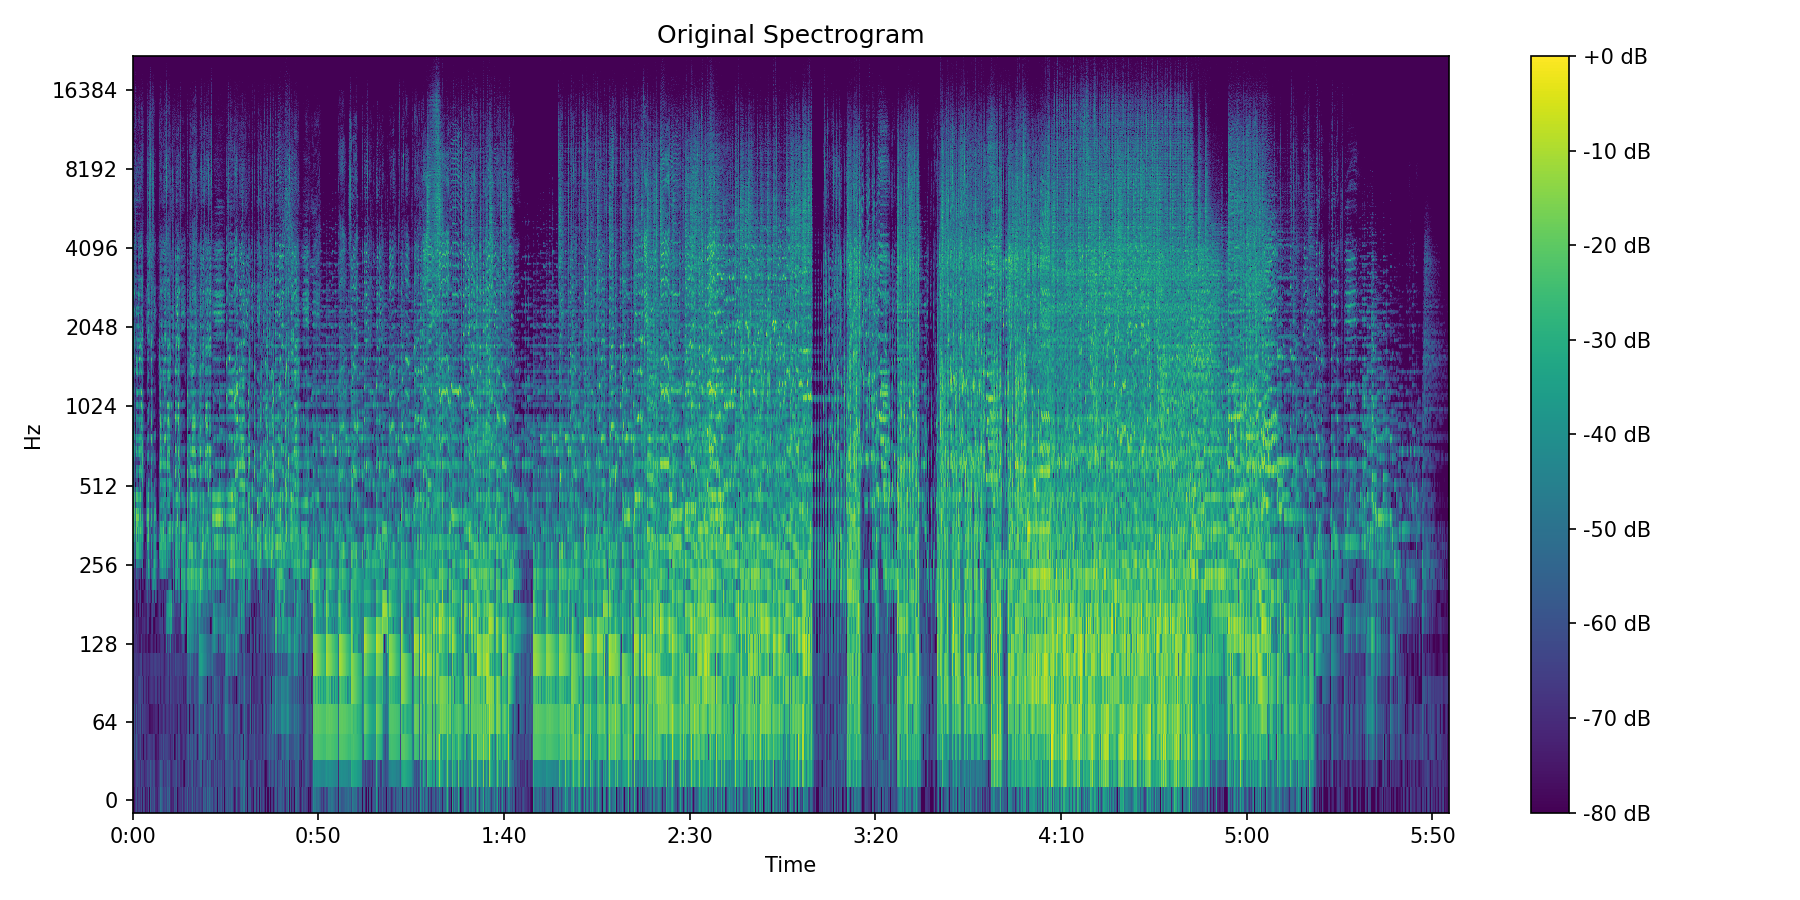
\includegraphics[width=0.9\textwidth]{spectrogram_original.png}
\end{figure}

\subsection{Spectograma aproximată}

\begin{figure}[h!]
    \centering
    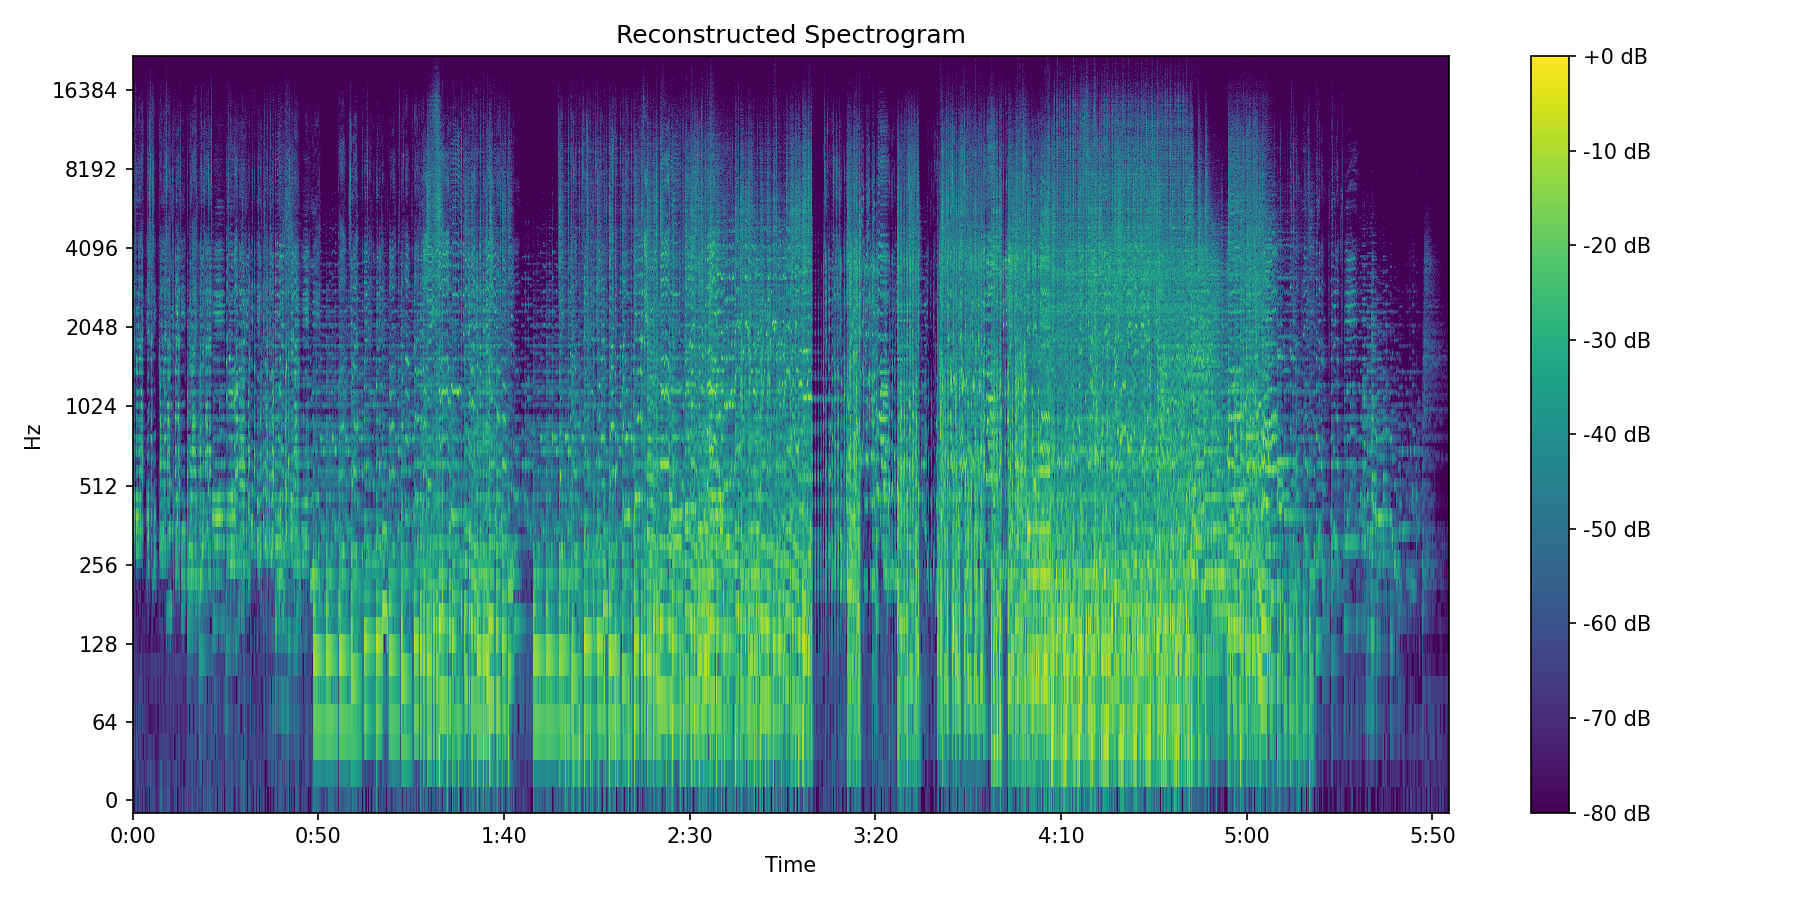
\includegraphics[width=0.9\textwidth]{spectrogram_reconstructed.png}
\end{figure}

\subsection{Spectograma originală 3D}

\begin{figure}[h!]
    \centering
    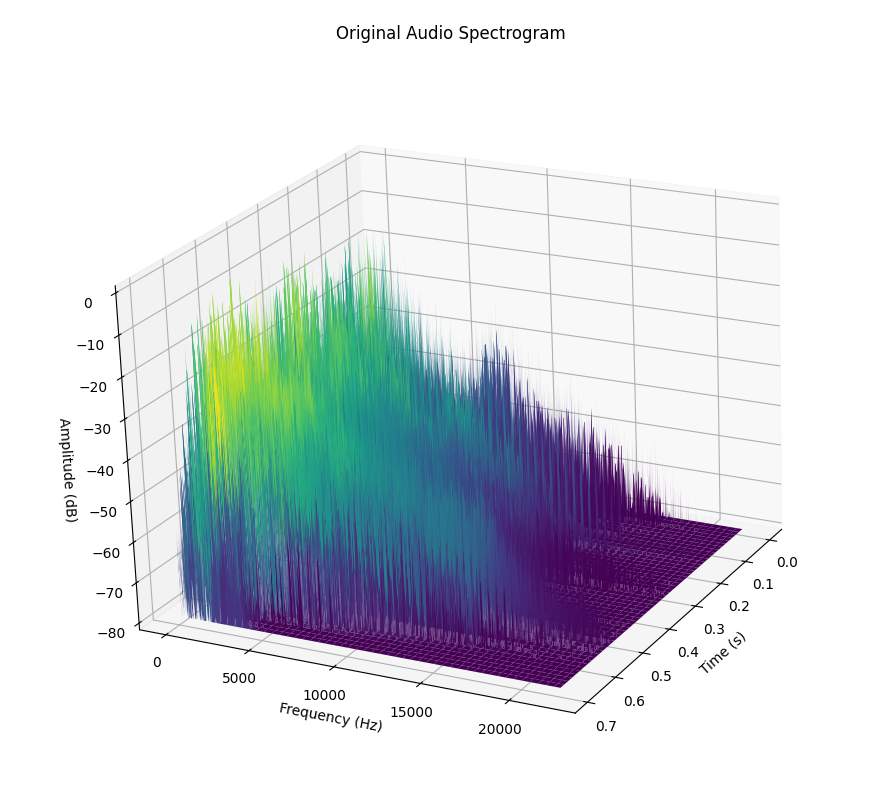
\includegraphics[width=0.6\textwidth]{3dog.png}
\end{figure}

\subsection{Spectograma aproximată 3D}

\begin{figure}[h!]
    \centering
    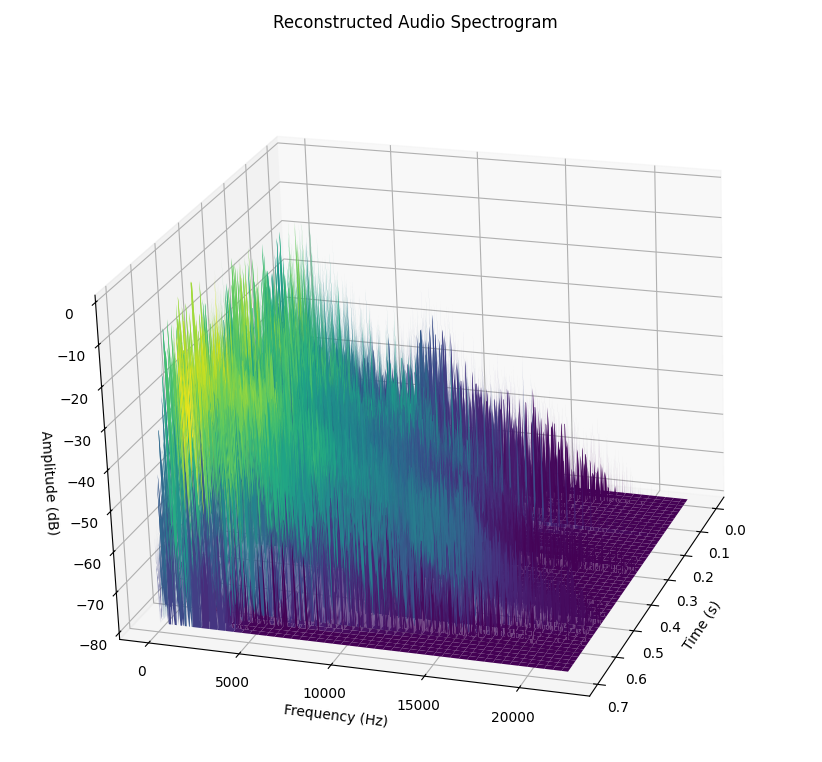
\includegraphics[width=0.6\textwidth]{3dap.png}
\end{figure}

\subsection{Grafice erori}

\begin{figure}[h!]
    \centering
    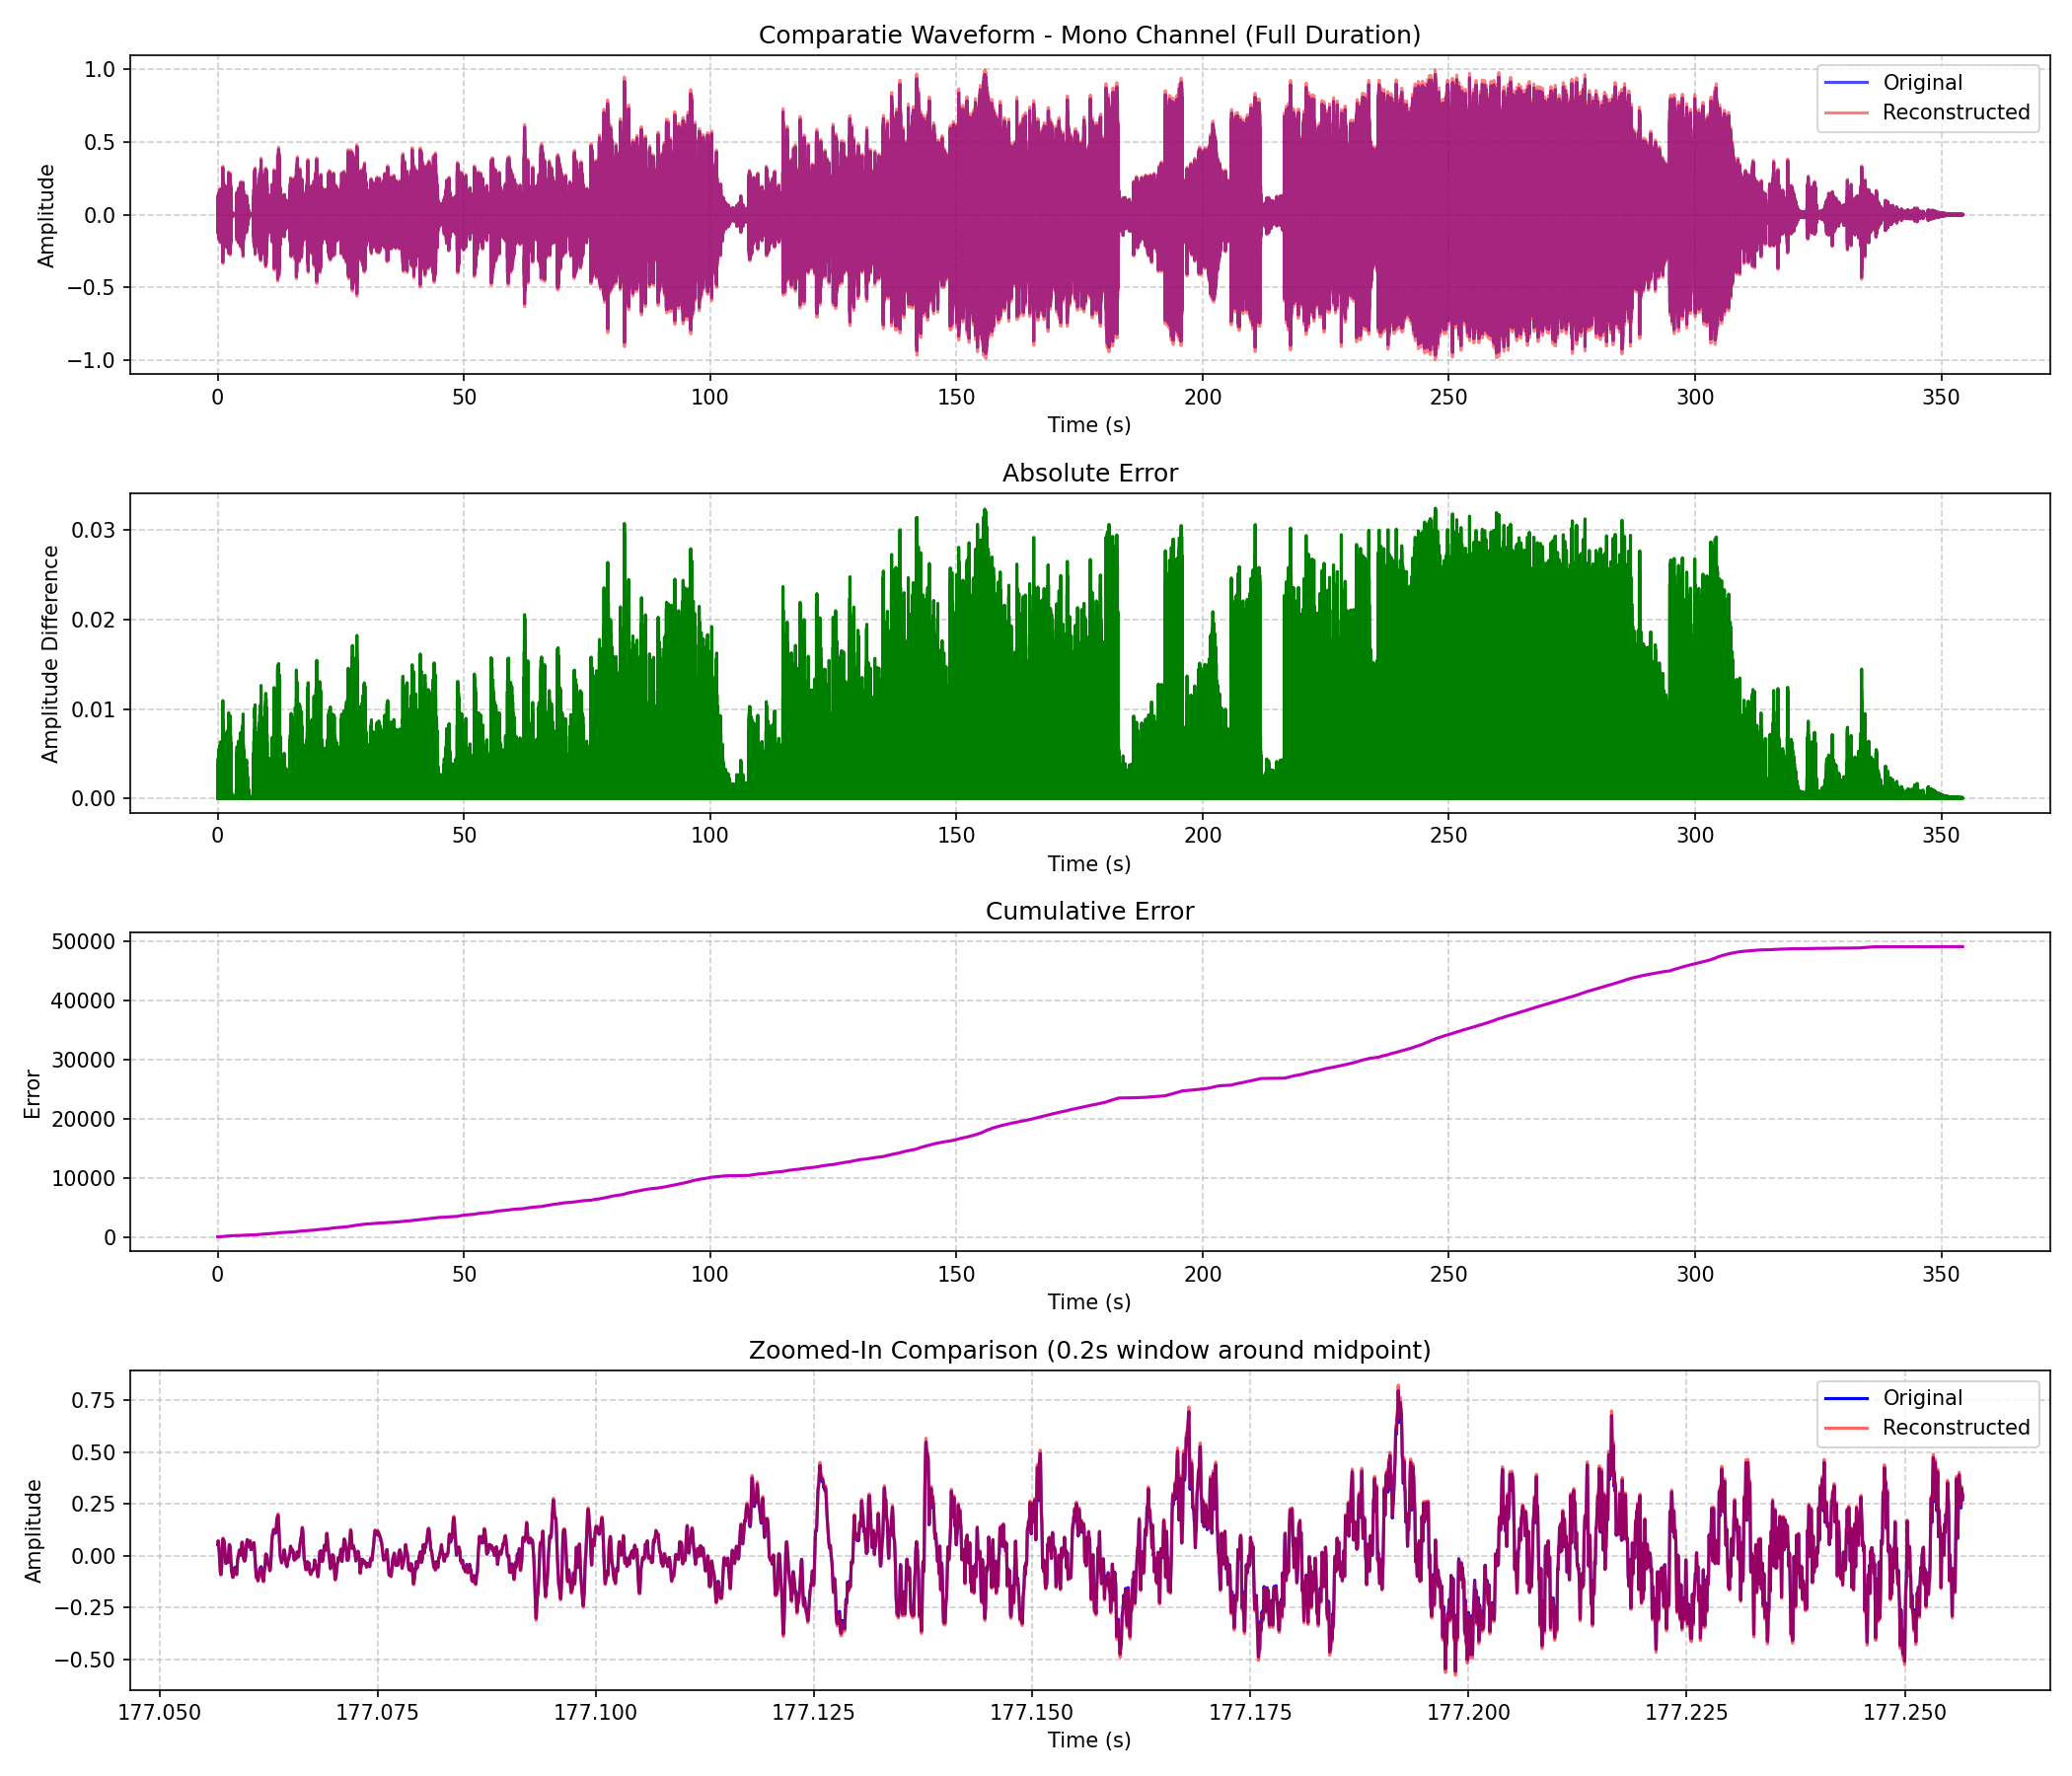
\includegraphics[width=1\textwidth]{waveform_comparison.png}
\end{figure}

\newpage

\subsection{Spectograma eroare}

\begin{figure}[h!]
    \centering
    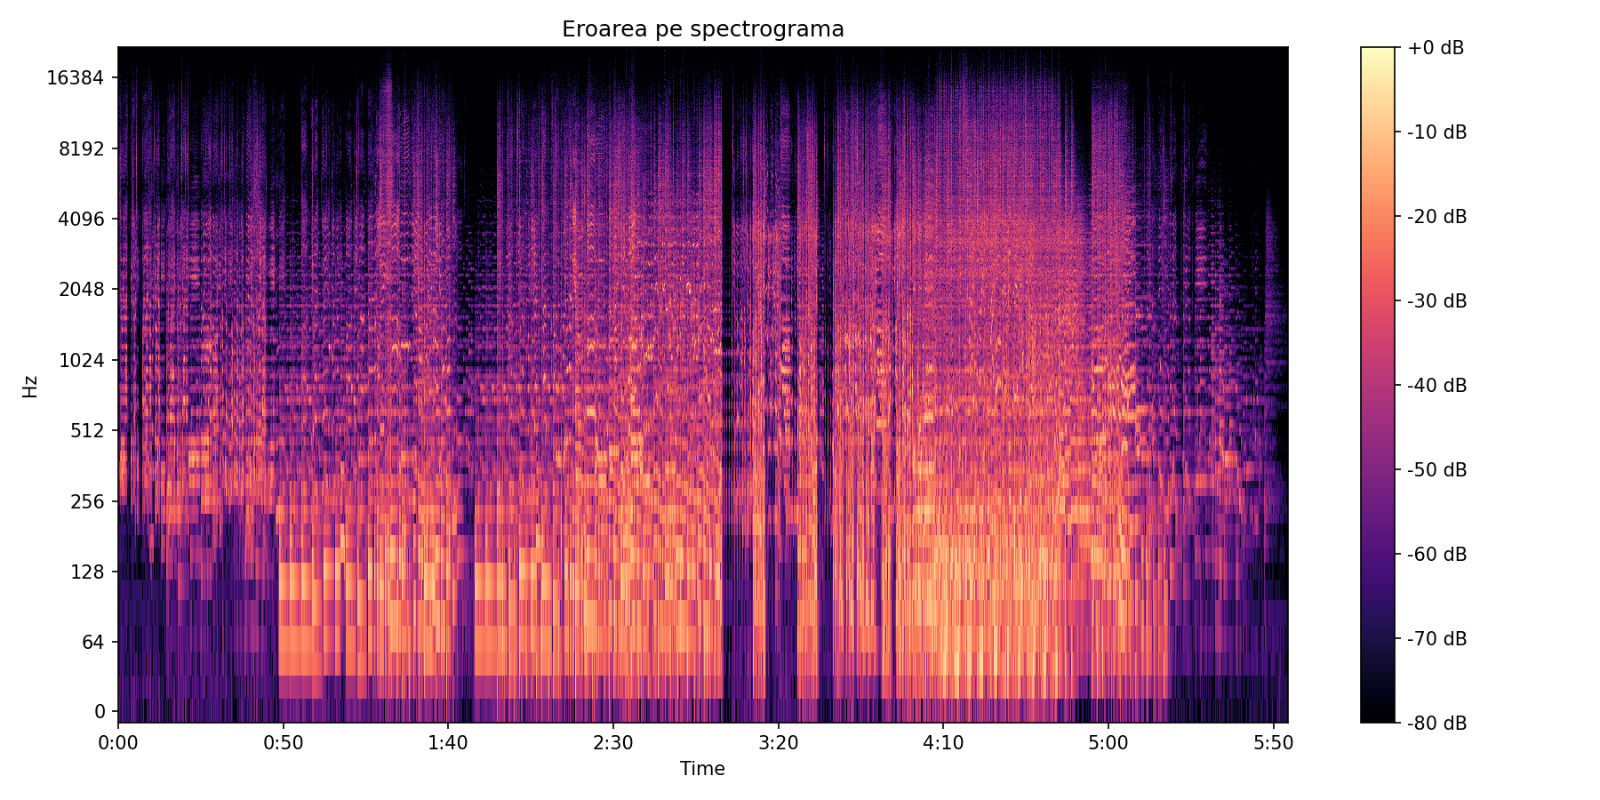
\includegraphics[width=1\textwidth]{spectograma_eroare.jpeg}
\end{figure}

\section{Bibliografia}

\begin{itemize}
    \item \href{https://www.pythonlikeyoumeanit.com/Module3_IntroducingNumpy/VectorizedOperations.html}{Vectorized Numpy Operations}
    \item \href{https://en.wikipedia.org/wiki/Cooley–Tukey_FFT_algorithm}{Cooley–Tukey FFT Algorithm}
    \item \href{https://numeric.cs.unibuc.ro/cn/cn-curs-6.pdf}{Curs CN - UNIBUC}
    \item \href{https://en.wikipedia.org/wiki/Singular_value_decomposition}{SVD - Wikipedia}
    \item \href{https://github.com/mich1803/SVD-Audio-Compression}{SVD Audio Compression - GitHub}
    \item \href{https://en.wikipedia.org/wiki/Spectrogram}{Spectrogram - Wikipedia}
    \item \href{https://en.wikipedia.org/wiki/Short-time_Fourier_transform}{STFT - Wikipedia}
    \item \href{https://en.wikipedia.org/wiki/Window_function#Hann_and_Hamming_windows}{Hann and Hamming Windows}
    \item \href{https://en.wikipedia.org/wiki/Uncertainty_principle}{Uncertainty principle}
    \item Ce a fost dezvăluit lui Robert cât timp visa
\end{itemize}

\end{document}
